

%\documentclass[conference]{IEEEtran}
%\IEEEoverridecommandlockouts
\documentclass{article}  
\twocolumn

\usepackage{graphicx}
\usepackage{caption}
\usepackage{algorithm}
\usepackage{algorithmic}
\usepackage{amsmath}
\usepackage{adjustbox}
\usepackage{authblk}
\usepackage{pbox}
\usepackage{float}
\usepackage[margin=1in]{geometry}
\author[1]{Dalia Ibrahim}
\author[2]{Carlos Dasaed Salcedo}


{
    \makeatletter
    \renewcommand\AB@affilsepx{: \protect\Affilfont}
    \makeatother
        
        

    \affil[ ]{Studnet ID}

    \makeatletter
    \renewcommand\AB@affilsepx{, \protect\Affilfont}
    \makeatother

    \affil[1]{201893217}
    \affil[2]{201892008}
    
        \makeatletter
\setlength{\floatsep}{5pt}
\setlength{\textfloatsep}{5pt}
    \makeatother
    
}

\begin{document}  

\title{ Assignment 2: Choosing the Best Parameters to Use for a Binary KNN classifier using on 5-fold cross-validation}


\maketitle
 \section{Introduction}
For this assignment, we have implemented a cross-fold validation algorithm from scratch using Python and the following libraries: pandas, numpy, math, random, and sys. To improve the efficiency of the algorithm, unsupervised filtering was also used based on the correlation matrix and variances of the data using sklearn libraries. The other sklearn libraries included in the final program were used to calculate KNN, and related precision metrics. To run the program, the following line must be executed from the command line in Linux: \\
\$python3 A2\_t2.py [DataFile.tsv]\\

 \section{ Preliminary Steps - Feature Selection }
feature selection\\
cross correlation\\
low variance \\

 \section{Main Pseudo-code}
This section only includes the functions that are relevant and currently being used by the algorithm. Functions, such as the ones from sklearn, will only be mentioned in the pseudo-code, but will not be individually described.
 \subsection{FoldSplitter()}

\begin{algorithm}[H]
\caption{Split Data in K folds}
\begin{algorithmic}[1]
\REQUIRE kfolds  \COMMENT{kfolds = 5 was used}
\STATE $ data \gets dataframe(DataFile.tsv)$
\STATE $ class0 \gets $ data.where(class=0).ShuffleRows() 
\STATE $ class0partition \gets  Rows In class0 / kfolds $
\STATE $ class1 \gets $ data.where(class=1).ShuffleRows()
\STATE $ class1partition \gets  Rows In class1 / kfolds $
\STATE $ leftOvers0 \gets $class0 rows after(class0partition * cvfolds)]
\STATE $ leftOvers1 \gets $class1 rows after(class1partition * cvfolds)]
\STATE $ leftOvers \gets  concatenation(leftOvers0,leftOvers1)$
\STATE $ theFolds \gets newPythonDictionary$
	\FOR { i=0 \textbf{to} kfolds-1 }
        \STATE  $create fold\textbf{i} $ \COMMENT{i = corresponding iteration in the for cycle} 
      	\STATE $class0Range \gets $class0[\textbf{from} i * class0partition \textbf{to} (i * class0partition)+class0partition  
      	\STATE $class1Range \gets$ class1[\textbf{from} i * class1partition \textbf{to} (i * class1partition)+class1partition   
      	\STATE $fold\textbf{i} \gets class0range + class1range  $
		\IF{$i = kfolds-1 $}
	  	\STATE $fold\textbf{i} \gets fold\textbf{i} + leftOvers $ 
		\ENDIF	
    \STATE $theFolds[fold\textbf{i}] = TempData $  	
	\ENDFOR
\STATE return theFolds 
\end{algorithmic}
\end{algorithm}

 \subsection{SplitData()}
\begin{algorithm}[H]
\caption{Create Learning and Training Data}
\begin{algorithmic}[1]
\REQUIRE DictionaryOfFolds , iterNum 
\STATE $ testFold \gets fold\{iterNum\}$ \COMMENT{iterNum refers to the iteration number, such that testFold will get fold1,fold2,...,fold5}
\STATE $testDF \gets DataFrame(testFold) $
\STATE $trainDF \gets NewDataFrame $
	\FOR { foldKey, foldValue \textbf{in} DictionaryOfFolds } 
		\IF{$foldkey = testFold $}
		  	\STATE Skip this Iteration 
		\ENDIF
        \STATE $trainDF.append(foldValue)$
  	\ENDFOR
\STATE $xtraining \gets $ trainDF without the last column 
\STATE $ytraining \gets $ testDF without the last column
\STATE $xtesting \gets $ trainDF with only the last column
\STATE $ytesting \gets $ testDF with only the last column
\STATE return xtraining, xtesting, ytraining, ytesting

\end{algorithmic}
\end{algorithm}


 \subsection{Calculate\_Nearest\_neighbour()}
 
\begin{algorithm}[H]
\caption{Calculate Nearest Neighbor Function}
\begin{algorithmic}[1]
\REQUIRE topMatched , K 
	%\IF{$topMatched[0].distance == 0 $}
	  %  \STATE $ FinalOutput \gets [topMatched.class, 1.00] $ 
	   % \STATE return FinalOutput
	%\ENDIF
	\STATE $TieBreaker \gets NewDataframe()$
	\STATE $TieBreaker \gets UniqueRandomNumbers()$
	\STATE $topMatched.CreateColumn('Count') \gets Count('Class')$
	\STATE $concatenate(topMatched, TieBreaker)$
	\STATE $topMatched = topMatched.Filter( 'Count' = Count.Max())$
	\STATE $topMatched.sortBy('tieBreaker')$
	\STATE $TopMatch \gets topMatched.row(0) $ 
	\STATE $Probability \gets \frac{topMatch[Count]}{ K}$
	\STATE $ FinalOutput \gets [TopMatch[Class], Probability)] $ 
    \STATE $return FinalOutput$
       
\end{algorithmic}
\end{algorithm}



\section{Deciding on Performance}  

Since there are several different performance metrics that can be used to determine how good an algorithm will perform, it is important to make an effort to chose an adequate performance metric for the task at hand. Upon inspection of the training data, it became obvious that the amount of zeros drastically outnumbered the amount of ones by ratio of about 10 to 1. This meant that blindly using accuracy as the factor to determine the best model would be insufficient, since an algorithm that always predicts the output class to be zero would actually be correct 90\% of the time. Therefore, to determine which model was best, we decided to focus on identifying instances of class 1. In other words, we considered ones as positive, and zeros as negatives to build the ROC curves, determine our loss function and select our best model \\



 \section{Results}
To validate the accuracy of our algorithm, we used the sklearn metrics library, which allowed us to generate image 1 and image 2
\begin{center}
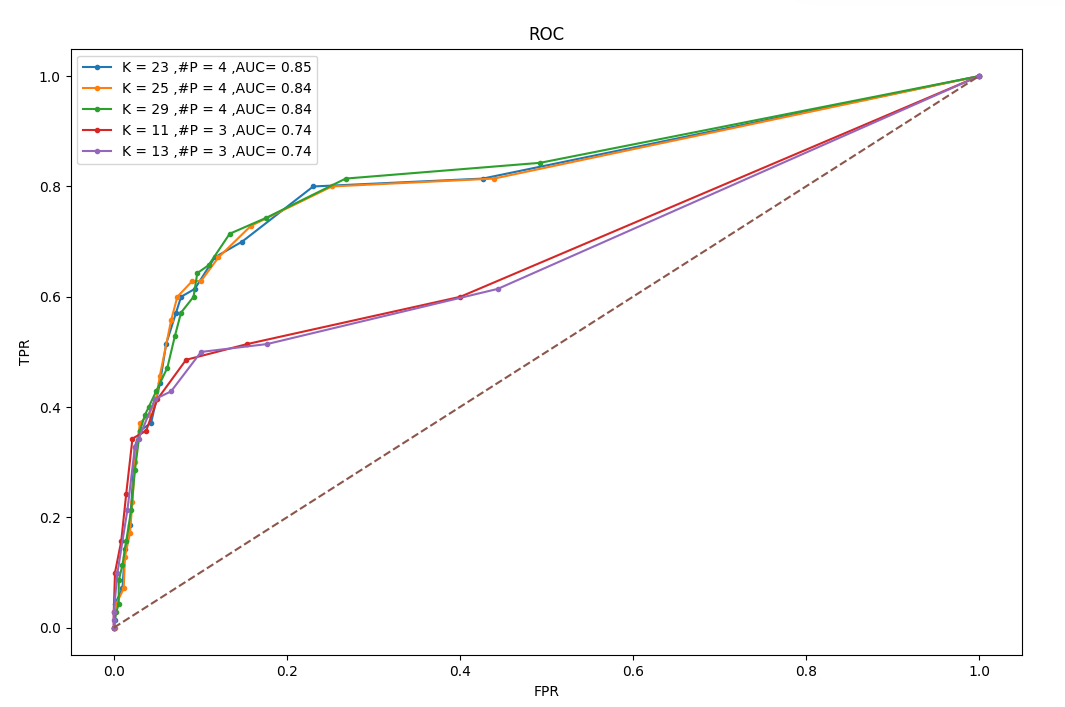
\includegraphics[scale=.2]{Roc2.png} 
\end{center}
Fig 1 ROC Curve for the 3 best models and the 2 worst models\\

\begin{center}
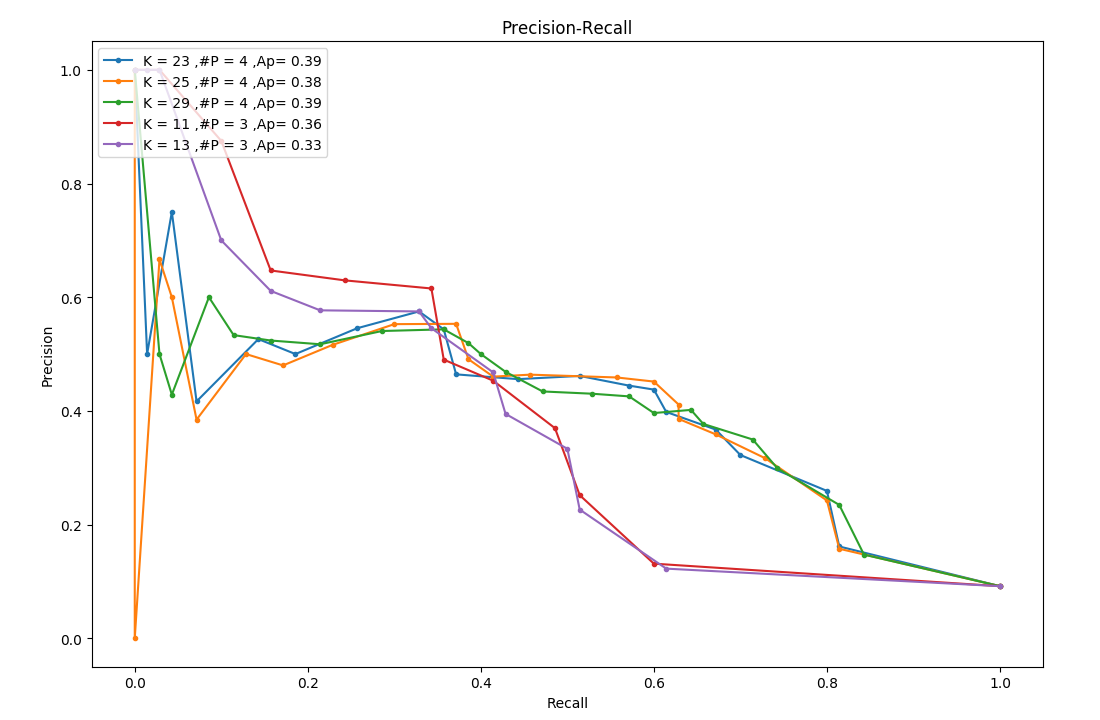
\includegraphics[scale=.2]{PR2.png}
\end{center}
Fig 2 Precision-Recall Curve for the 3 best models and the 2 worst models


\section{Conclusion}
KNN is a powerful and useful machine learning classifier. However, just like any other classifier, without the proper parameters such as an adequate feature selection, number of neighbors, and correct training set, the model can easily become skewed or flawed. For this reason, it is important to select the proper performance metrics and to run cross validation tests with at least 5 folds. In our particular case, using 5 fold cross validation, and selecting the features based on a correlation matrix and variance, consistent models with AUCs of up to 0.85 were obtained.   \\ 
 
 

\end{document}
